\documentclass[10pt,a4paper]{article}

\usepackage[utf8]{inputenc}
\usepackage[T1]{fontenc}	
\usepackage[italian]{babel}
\usepackage{amsmath}
\usepackage{amsfonts}
\usepackage{amssymb}
\usepackage{graphicx}

\usepackage[left=2cm,right=2cm,top=2cm,bottom=2cm]{geometry}
\geometry{a4paper}

\usepackage{booktabs} % for much better looking tables
\usepackage{verbatim}
\usepackage{subfig} % make it possible to include more than one captioned figure/table in a single 

\usepackage{fancyhdr} % This should be set AFTER setting up the page geometry
\pagestyle{fancy} % options: empty , plain , fancy
\renewcommand{\headrulewidth}{0pt} % customise the layout...
\lhead{}\chead{}\rhead{}
\lfoot{}\cfoot{\thepage}\rfoot{}

%%% SECTION TITLE APPEARANCE
\usepackage{sectsty}
%\allsectionsfont{\sffamily\mdseries\upshape} % (See the fntguide.pdf for font help)
% (This matches ConTeXt defaults)

% pacchetti che mi fanno schifo ma uso lo stesso
\usepackage[cdot, thickqspace]{SIunits}
% macro che mi piacciono
\def\code#1{\texttt{#1}}

\title{Esercitazione 3: Misure DC su transistor e NOT TTL}

\author{Gruppo BE \\ Alessandro Candido, Roberto Ribatti}
\date{\today}
\begin{document}
\maketitle

\section{Scopo e strumentazione}

\section{Misure in DC sul transistor}
Si è proceduto alla realizzazione del circuito in figura \figurename{\ref{circuito}} e si sono utilizzate le seguenti componenti:
\begin{figure}[h!]
\begin{minipage}[c]{0.5\textwidth}
\begin{align*}
R_L &= \unit{989 \pm 9}{\ohm}\\
R_B &= \unit{46.4 \pm 0.5}{\kilo\ohm}\\
R_{trim} &= \unit{101.5 \pm 0.9}{\kilo \ohm}\\
V_1 &= \unit{9.84 \pm 0.4}{\volt}\\
\end{align*}
	\end{minipage}
	\begin{minipage}[c]{0.5\textwidth}
	\centering
	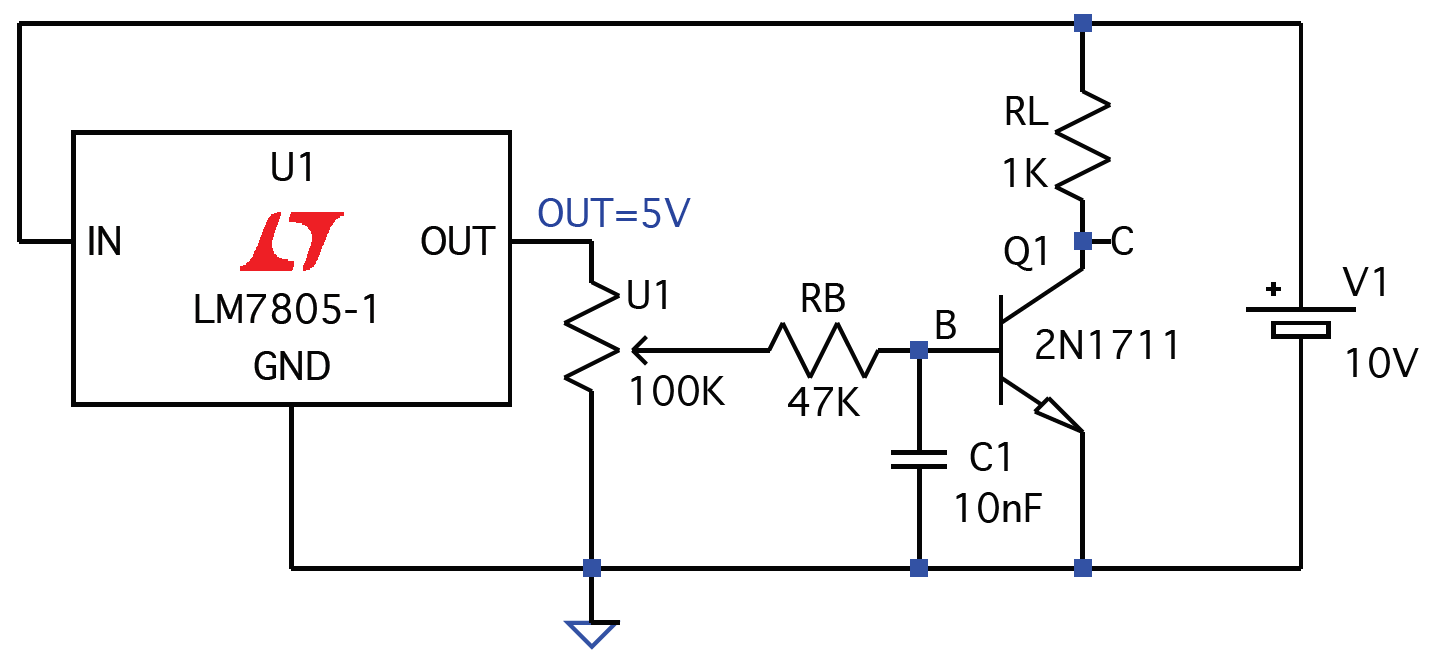
\includegraphics[width=0.8\textwidth]{../grafici/circuito.png}
	\caption{Circuito realizzato}
	\label{circuito}
	\end{minipage}
\end{figure}

\subsection{Retta di carico}
Si è tracciata la retta di carico sul grafico $I_c/V_{CE}$ fornito e si sono identificate le zone di interdizione (in basso), saturazione (a sinistra) e la zona attiva (il resto del grafico).
\begin{figure}[h]
	\centering
	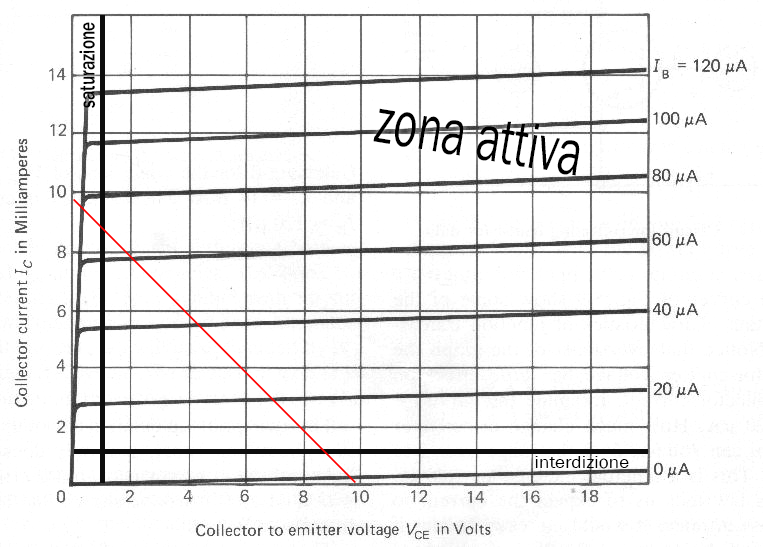
\includegraphics[width=0.6\textwidth]{../grafici/retta_carico.png}
	\caption{Retta di carico e zone di lavoro del transistor}
	\label{retta_carico}
\end{figure}
\subsection{Variando $I_b$} %da cambiare
Si è proceduto alla misura di 3 tensioni al variare della posizione del potenziometro:
\begin{itemize}
	\item tensione base/emettitore $V_{BE}$ (misurata con l'oscilloscopio)
	\item tensione collettore emettitore $V_{CE}$ (misurata con l'oscilloscopio), a partire dalla quale, nota la tensione di alimentazione $V_1$, si è calcolata la caduta di potenziale su $R_L$ e di conseguenza la corrente di collettore $I_C$;
	\item caduta di tensione su $R_B$ (misurata con il multimetro), con la quale si è calcolata la corrente di base $I_B$.
\end{itemize}
Si sono graficate la corrente di collettore $I_C$ in funzione della corrente di base $I_B$ e della tensione base/emettitore $V_{CE}$.
Di seguito riportiamo i dati raccolti e i grafici realizzati.

\begin{figure}[h!]
	\centering
	\begin{minipage}[h!]{0.4\textwidth}
		\centering
		\resizebox{1\textwidth}{!}{
			\input{../tabelle/tab_ib_var.txt}}
		\captionof{table}{Dati raccolti}
	\end{minipage}
	\begin{minipage}[d]{0.59\textwidth}
		\centering
		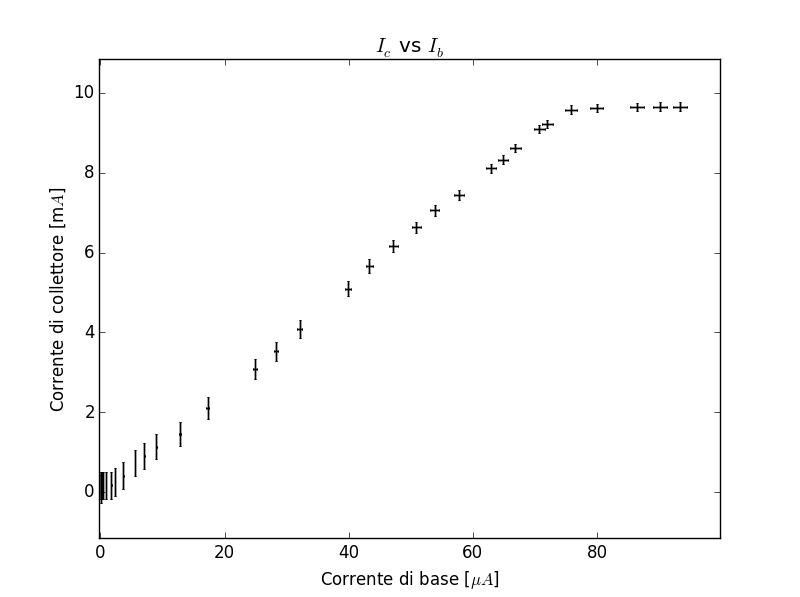
\includegraphics[width=1.1\textwidth]{../grafici/ic_ib.pdf}
		\caption{Grafico corrente collettore vs corrente di base}
		\label{ibic}
		\centering
		\includegraphics[width=1.1\textwidth]{../grafici/ic_vbe.pdf}
		\caption{Grafico tensione BE vs corrente collettore}
		\label{vbeic}
		\end{minipage}
\end{figure}

Variare la posizione del potenziometro non cambia la retta di carico ma modifica la corrente di base, quindi cambia la curva la curva la cui intersezione con la retta di carico produce il punto di lavoro del transistor.
Il grafico in \figurename{\ref{ibic}} può essere suddiviso in tre parti:
\begin{itemize}
	\item i punti addensati vicino allo $0$ sono le intersezioni della retta di carico con le curve a corrente di base $\sim \unit{ 0}{\micro\ampere}$ (zona di interdizione);
	\item nella zona centrale è chiaro un andamento lineare, interrotto per correnti di base $>\unit{80}{\micro\ampere}$, in questa zona la retta di carico interseca le curve in zona attiva ed è verificata l'ipotesi di linearità attesa: $I_C = h_{FE}*I_B$;
	\item per valori di corrente di base $>\unit{80}{\micro\ampere}$, il grafico abbandona l'andamento lineare della zona centrale e si stabilizza sul valore di $V_{CE}(sat)$: per grandi variazioni di corrente di base non corrispondo significative variazioni di corrente di collettore: in questa zona la retta di carico interseca le curve in zona di saturazione. Come è visibile in \figurename{\ref{retta_carico}} superati gli $\unit{80}{\micro\ampere}$ le curve intersecano la retta di carico circa nello stesso punto.
\end{itemize}
La massima corrente erogabile dal transistor è $I_{max}=V_1/R_L$\footnote{stiamo trascurando la resistenza del transistor poichè siamo in regime di saturazione}, con gli attuali parametri otteniamo $I_{max}=\unit{9.9 \pm 0.1}{\milli\ampere}$. 

Per stimare la tensione di saturazione $V_{CE}(sat)$ faccio una media pesata dei punti presi in regime di saturazione e ottengo $V_{CE}(sat)$=\unit{298 \pm 5}{\milli\volt}.

Si è eseguito un fit lineare\footnote{che tenesse conto anche dell'errore sulle ascisse, che per certi dati è paragonabile a quello sulle ordinate} della zona centrale per il calcolo del parametro $h_{FE}$, il cui risultato è stato:
\begin{equation*}
h_{FE} = 130.1 \pm 2.2
\end{equation*}
\begin{figure}[h!]
	\centering
	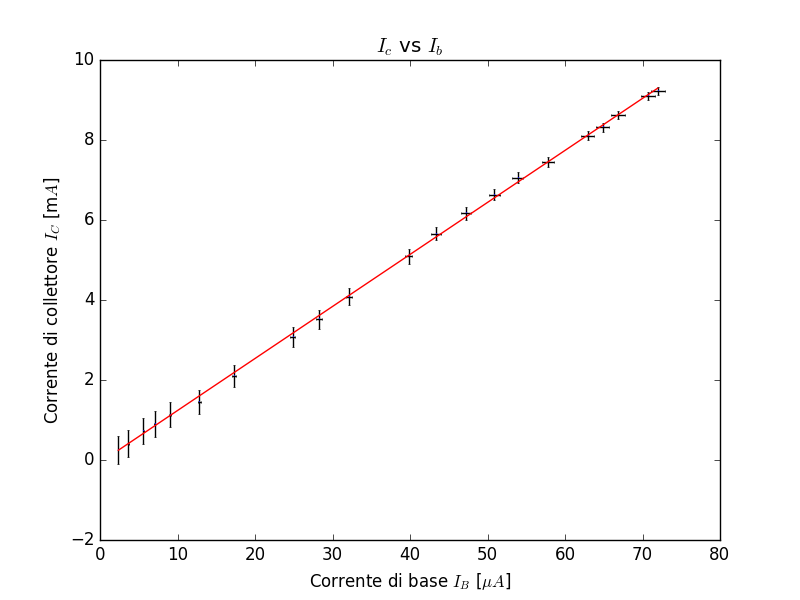
\includegraphics[width=0.6\textwidth]{../grafici/fit_h_fe.pdf}
	\caption{Grafico del fit di $h_{FE}$}
\end{figure}

Il grafico in \figurename{\ref{vbeic}} può essere diviso in due zone:
\begin{itemize}
	\item un plateau fino alla tensione di $\unit{600}{\milli\volt}$, in questa zona troviamo i punti che nel grafico in \figurename{\ref{vbeic}} erano addensati vicino allo $0$, ovvero quelli i punti di intersezione tra retta di carico e curve nella zona di interdizione.
	\item una retta molto pendente (o volendo un esponenziale in base al grado di approssimazione) che parte come ci si aspetterebbe per $V_{BE} \sim \unit{0.7}{\volt}$, ovvero quando il transistor passa in zona attiva e la giunzione BE risulta polarizzata.
\end{itemize}

\subsection{Variando $V_{CE}$}
Si fissa adesso la posizione del potenziometro in modo da avere una corrente di base di $\sim \unit{40}{\micro\ampere}$. Si procede alla misura della tensione collettore emettitore $V_{CE}$ e della tensione di alimentazione $V_1$ al variare di quest'ultima in un range tra $\unit{6}{\volt}$ e $\unit{15}{\volt}$.

Di seguito il grafico della corrente di collettore $I_C$\footnote{si è calcolata la caduta di tensione sulla resistenza $R_L$ per differenza delle due tensioni misurate} in funzione della tensione collettore/emettitore $V_{CE}$.

\begin{figure}[h!]
	\centering
	\begin{minipage}[h!]{0.3\textwidth}
		\centering
		\resizebox{\textwidth}{!}{
			\input{../tabelle/tab_Early.txt}}
		\captionof{table}{Dati raccolti}
	\end{minipage}
	\begin{minipage}[d]{0.69\textwidth}
		\centering
		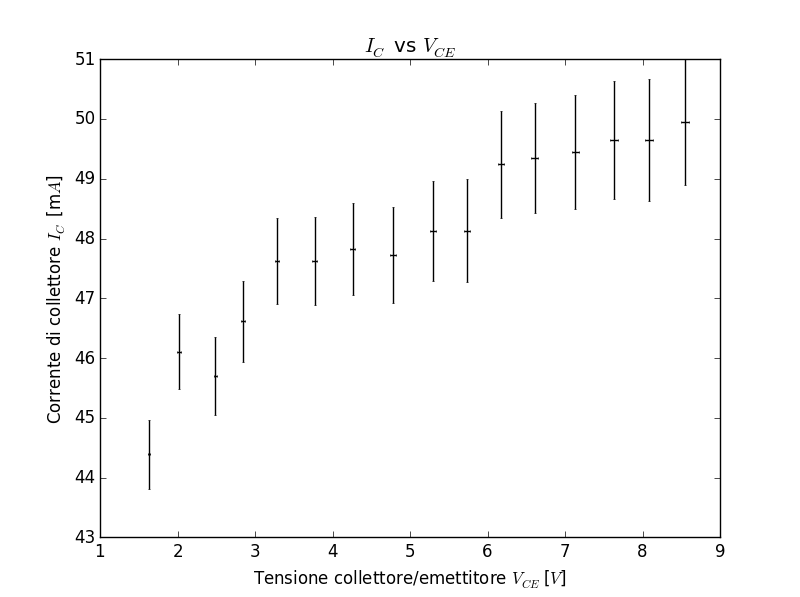
\includegraphics[width=\textwidth]{../grafici/fast_plot_early.pdf}
		\caption{Grafico effetto Early}
		\label{early}
	\end{minipage}
\end{figure}

Al variare della tensione di alimentazione $V_1$ la retta di carico si muove parallelamente a se stessa su grafico come in \figurename{\ref{retta_spostamento}}, quindi spostandosi la retta di carico interseca diversi punti della curva a  $\sim \unit{40}{\micro\ampere}$, il risultato e il caratteristico andamento lineare prodotto dall'effetto Early, come si nota anche dalle misure graficate in \figurename{\ref{early}}.

\begin{figure}[h!]
	\centering
	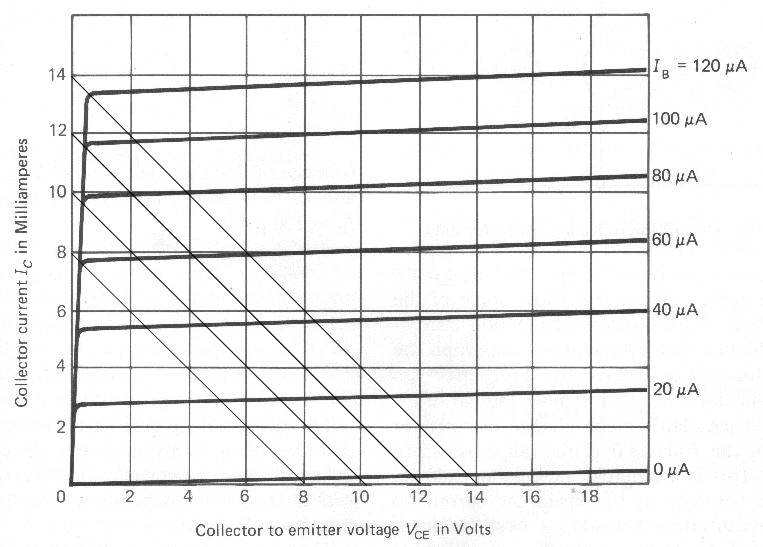
\includegraphics[width=0.6\textwidth]{../grafici/spostamento_retta.jpg}
	\caption{Variazione della retta di carico}
	\label{retta_spostamento}
\end{figure}

\section{Circuito NOT}

\subsection{Porta NOT}
\begin{figure}[h!]
	\centering
	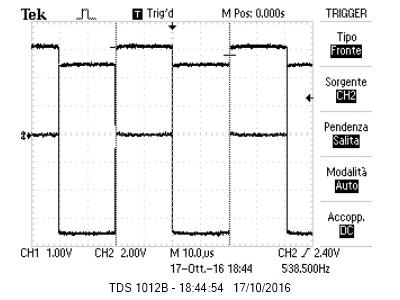
\includegraphics[width=0.6\textwidth]{../oscilloscopio/not_tarocco.jpg}
	\caption{}
\end{figure}
% se torniamo in lab prendiamo una schermata del funzionamento come porta NOT dall'oscilloscopio
Si è costrituito il circuito riportato sulla scheda con i seguenti valori per le resistenze:

\begin{table}[h!]
\centering
\begin{tabular}{c|c|c}
$R_1 = \unit{15.20 \pm 0.13}{\kilo\ohm}$ & $R_2 = \unit{99.4 \pm 0.9}{\kilo\ohm}$ & $R_L = \unit{2.27 \pm 0.03}{\kilo\ohm}$
\end{tabular}
\end{table}

Si sono quindi misurati i seguenti valori per gli stati \code{alto} e \code{basso} di $V_{out}$ e $V_{in}$:

\begin{table}[h!]
\centering
\begin{tabular}{c|c|c}
 & $V_{in}$ [mV]& $V_{out}$ [V]\\
\code{alto} & $668 \pm 4$ & $5.12 \pm 0.04$\\
\code{basso} & $0.24 \pm 0.10$ & $0.0576 \pm 0.0004$
\end{tabular}
\end{table}

Da cui si ottengono le correnti:

\begin{table}[h!]
\centering
\begin{tabular}{c|c|c}
 & $I_B$ [mV]& $I_C$ [V]\\
\code{alto} & $$ & $$\\
\code{basso} & $$ & $$
\end{tabular}
\end{table}

\subsection{Ritardi}
Si è analizzato il comportamento del circuito su una scala temporale più piccola rispetto al periodo del segnale. Si nota che:
\begin{itemize}
\item il circuito produce un uscita non perfettamente in fase con l'ingresso;
\item l'onda quadra in uscita risulta non avere più un netto fronte di salita, ma impiega un tempo non indifferente per cambiare stato.
\end{itemize}

Si sono misurati i tempi caratterisci, relativi ad una frequenza di input pari a $f = \unit{551.7 \pm}{\hertz}$, che vengono riportati di seguito. I nomi sono usati conformemente alla scheda relativa all'esercitazione. 

\begin{table}[h!]
\centering
\begin{tabular}{c|c|c|c}
$T_{rs} = \unit{264 \pm 5}{\nano\second}$ & $T_{s} = \unit{328 \pm 5}{\nano\second}$ & $T_{rd} = \unit{10.1 \pm 0.3}{\micro\second}$ & $T_{d} = \unit{1.98 \pm 0.03}{\micro\second}$
% ho inserito come errori solo gli 0.1DIV, non ricordo se vogliamo inserire anche una tacca/mezza-tacca addizionale del cursore in quadratura, oppure se in qualche misura c'era un po' di errore dovuto all'oscillazione della traccia
\end{tabular}
\caption{Tempi caratterisci del segnale in uscita dalla porta NOT}
\end{table}


\paragraph{Discrepanza salita-discesa} Si nota che i tempi di discesa sono ordini di grandezza più grandi di quelli di salita. Si ricercano le cause di questa discrepanza nel funzionamento del transistor, e osservando il grafico $V_{CE} - I_C$ si nota che per compiere anche piccole variazioni di tensione lungo la retta di carico:
\begin{itemize}
\item per grandi tensioni $V_{CE}$, cioè in interdizione, il comportamento è quasi lineare, come in regime attivo;
\item per piccole tensioni $V_{CE}$, cioè in saturazione, per ottenere piccole variazioni sono necessarie grosse variazioni di $I_B$.
\end{itemize}
Si suppone che la variazione di $I_B$, che dovrebbe essere in fase con quella di $V_{in}$ (proveniente da \code{OUTPUT PULSE}), ma tenendo conto di ciò si giustifica una differenza di tempi fra la parte vicina al basso sia della salita che della discesa, ma non la più evidente differenza tra i due.



Nei due casi si ha che:
\begin{description}
\item[salita] Il transistor deve transistare dallo stato alto allo stato basso, perciò deve passare da interdizione a saturazione. Quindi...
\item[discesa] Al contrario rispetto al caso precedente si deve passare da saturazione a interdizione.
\end{description}

\subsection{Resistenza $R_2$}

\subsection{Limiti del circuito in frequenza}

\begin{figure}[h!]
\centering
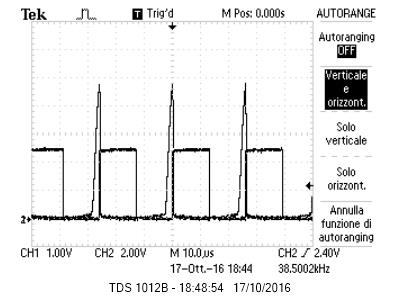
\includegraphics{../oscilloscopio/raise_problem.jpg}
\caption{}
\end{figure}

\end{document}
